\documentclass[10pt,twocolumn]{article}
\usepackage{times}
\usepackage{graphicx}
\usepackage{amssymb}
\usepackage{titling}
\usepackage{url,hyperref}

\begin{document}

\title{\LaTeX\ Detecting Fraudulent Universities}

\author{Michelle Ho and Shay Lehmann}

\date{%
CUSP-GX-5006\\
Machine Learning Final Project \\
\rule{\textwidth}{1pt}
}

\posttitle{\par\rule{3in}{0.4pt}\end{center}\vskip 0.5em}
%\postdate{\rule{\textwidth}{1pt}}

\maketitle

\begin{abstract}

For this project, the authors sought to examine higher education in the United States
using the College Scorecard dataset. Their goals were twofold: 1) predict an
institution's default rate for given data on the cohort and 2) proactively identify
potentially fraudulent schools.

\end{abstract}


\section{Introduction}

In the United States, the rising cost of a college degree and the corresponding
increase in student loans is well-documented. Nonetheless, a college degree is the bare
minimum requirement for many positions regardless of whether the specific major
has provided any subject matter expertise relevant to the industry. The authors
initially set out to identify the 'best value' colleges and set upon the rate of
student loan default on federally-funded loans as the metric with which to define
value. Default is perhaps the worst possible outcome of a university education
as the borrower likely has not been able to obtain a well-paying job, but instead
has a loan that they cannot afford to pay off. The default will then have a
detrimental affect on credit history for years to come. Exploratory analysis
revealed significant discrepancies in the distribution of loan default by
institution type, with public and private not-for-profit schools exhibiting similar
patterns. Private for-profit schools, on the other hand, exhibited a significantly
higher mean default rate as well as a much larger range of potential outcomes with
some schools reaching default rates over 30% (See Figure 1). The authors then
began a secondary inquiry to determine whether they could identify fraudulent or
potentially fraudulent universities. A number of for-profit universities, including
Corinthian College have recently come under investigation by the Federal Government
for their graduates' high default rates. These universities have been found to have
misled students on their potential job prospects after graduation. In many instances,
the Federal Government has forgiven several millions of dollars in outstanding loans.
While loan forgiveness is one step towards aiding the victims of these universities,
these graduates have likely not received an adequate education and have likely not
found their job prospects improved. Additionally, this is expensive for taxpayers
who have underwritten worthless educations.

The authors hope machine learning techniques can be used to identify a school's
loan default rate and, particularly, those which are fraudulent. They hope that this
will enable the government to take proactive steps towards investigating such universities
before they are able to collect years of federal funds while delivering low quality
education. They also hope that publicizing the high default rates will prompt
reform of the process and build support for increased funding for public universities.


\section{Methods and Data Sets}
This report makes use of the College Scorecard dataset. This dataset is a compilation
of education-related measurements, as collected by a number of federal institutions
from the Department of Education to the Treasury Department. This is a relatively new
initiative to centralize disparate agencies measurements into one location so
although data goes back to the 1990s, many years do not have data for all variables.
As such, the authors examined data from the 2011-2013 cohorts in order to predict the 3-year
default rate for the cohort. This dataset includes 7414 schools and 1743 variables.
However, there is not complete coverage for all variables depending on the
institution. For this analysis, the data was subsetted based upon available
features.

The variables are described below:

\item \texttt{CONTROL}: a categorical variable indicating the funding type of a school.
Categories are 1=``public", 2=``private non-profit", or 3=``private for-profit".
\item \texttt{CDR3}: Cohort Default Rate at 3 Years
\item \texttt{MAIN}: Boolean identifier for main campus
\item \texttt{LO\char`_INC\char`_DEBT\char`_MDN}: The median debt for students with family income between \$0-\$30,000
\item \texttt{HI\char`_INC\char`_DEBT\char`_MDN}: The median debt for students with family income \$75,001+
\item \texttt{MD\char`_INC\char`_DEBT\char`_MDN}: The median debt for students with family income between \$30,001-\$75,000
\item \texttt{FIRST\char`_GEN}: Share of students who are first-generation students
\item \texttt{COMP\char`_ORIGIN\char`_YR4_RT}:  Share of students who complete at the original university within 4 years
\item \texttt{ADM\char`_RATE\char`_ALL}: The admissions rate for the entire school
\item \texttt{AGE\char`_ENTRY}: The average age at time of entry for students
\item \texttt{INEXPFTE}: Dollars spent by the institution on education per full-time student
\item The dependent variable being classified and predicted is `CDR3' for the first step.
\item The data was limited to only the main campus for each institution as many features
were reported as identical for each satellite campus leading to redundant entries.
The MAIN column was then dropped for further analysis.
\item The independent variables are all the others.
\item Any observations with null values for any of the chosen variables
are dropped. After these drops, the number of observations
in the dataset is 2122 for the 2011 cohort, 2151 for the 2012 cohort, 2052 for the
2013 cohort.
\item Finally, the categorical variable \texttt{CONTROL} is binarized so that all samples
are represented by boolean feature vectors.
\end{itemize}


\end{enumerate}

\section{Results}

3-Year Default Rate for the cohort was then predicted using Random Forest Regression
from the SKlearn package on test samples of size 25%, 33%, 50%, 67% and 75% for each cohort with
a random_state = 23. Additionally, a varied set of max_depths were tested on the 2011
cohort to identify how changing the depth affected the model. Maxes of 3, 5, 8 and 11 were
 tested with a test sample of 33%. The in-sample and out-of-sample R^2 as well as
 the important features were reported for each
model and the resulting prediction versus actual were visualized. The various models
had similar predictive capabilities within their cohort. For instance, the model
trained on 67% of the data for the 2011 cohort with a max depth of 8 had an in-sample R^2 of .917 with an
out-of-sample R^2 of .789. This model identified the most important feature as the
share of first generation students (52.7% of models), followed by median debt for
students with medium level family income (13.7%), the percent of students completing
within 4 years at the original university (10.1%) and whether a private for-profit
university (8%). The visualization of actual versus predicted can be seen in Figure 2.
A model built on 2012 cohort data yielded an insample R^2 of .911 and an out-of-sample R^2
of .818. This model once again identified the share of first generation students as most important
(52.4%) and the percent completing at the original school (24.3%). No other features
were in over 10% of models. The 2013 dataset yielded slightly different levels of importance with
an R^2 of .903 in sample and an R^2 of .741 out-of-sample. However, important features
were identified as the percent completing at the original institution (47.7%) followed by
percent first generation (22.4%) and whether private not-for-profit (10.5%).

Given the variety from year to year, the authors attempted to validate a model
trained on 2011 data with results from 2013. The debt variables and the dollar
amount spent on instruction per student were thus scaled have a mean of 0 and a standard
deviation of 1 in order to account for changes in attendance cost. However, the
model did not seem to work from year to year as the out of sample R^2 was only .547. The
visualization suggests that default rates were actually over-predicted for many in the
cohort.

Lastly, the authors created a model based on an average of the prior two years, 2011
and 2012 to test 2013 data. This model was built by averaging the features over years
2011 and 2012 in order to test 2013 data. This model performed fairly well, with
an in-sample R^2 of .896 and an out-of-sample R^2 of .722. The average share of
first generation students and the average completion rate were again pointed to
as important features. However, previous cohorts do not have the same data available
so it is unclear whether an averaged model would work in subsequent years.

Lastly, a brief examination was done on the effect of max_depth of tree against
reliability of results. For the 2011 cohort, the max depth of the trees were tested
for a range of 3 to 11. While in-sample R^2 increased regardless of depth, out-of-sample
R^2 plateaued around a depth of 8, indicating an overfitting problem. As such, a depth of 8
was used for analysis.




    ~\ref{results2011}.

\begin{figure}[!t]
  \begin{center}
    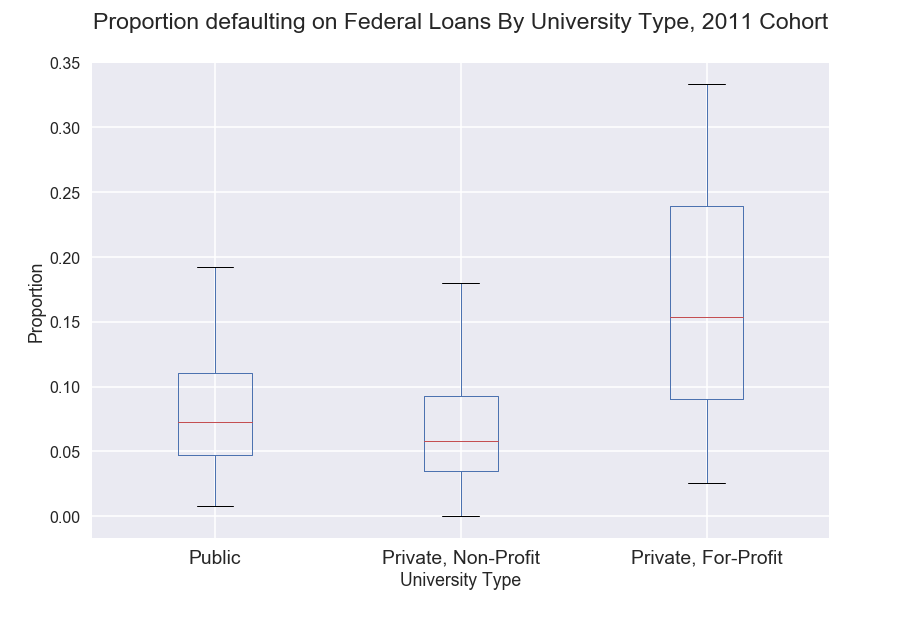
\includegraphics[width=2.5in]{fedloans.png}
  \end{center}

  \caption{\Figure 1: Exploratory look at difference between default rates by Control Group, 2011}
  \label{boxplot}
\end{figure}

\begin{figure}[!t]
  \begin{center}
    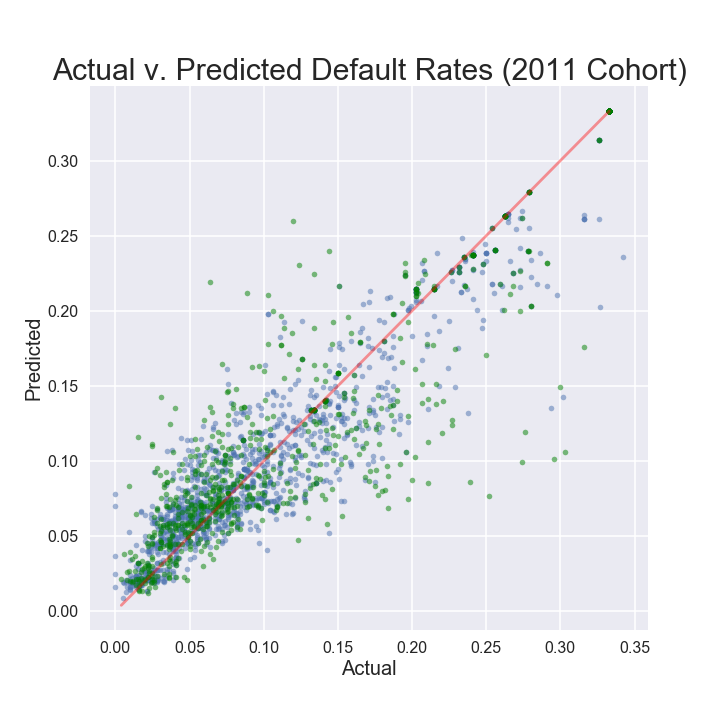
\includegraphics[width=2.5in]{results2011.png}
  \end{center}

  \caption{\Figure 2: Results of the model trained on data from the 2011 cohort}
  \label{results2011}
\end{figure}

\begin{figure}[!t]
  \begin{center}
    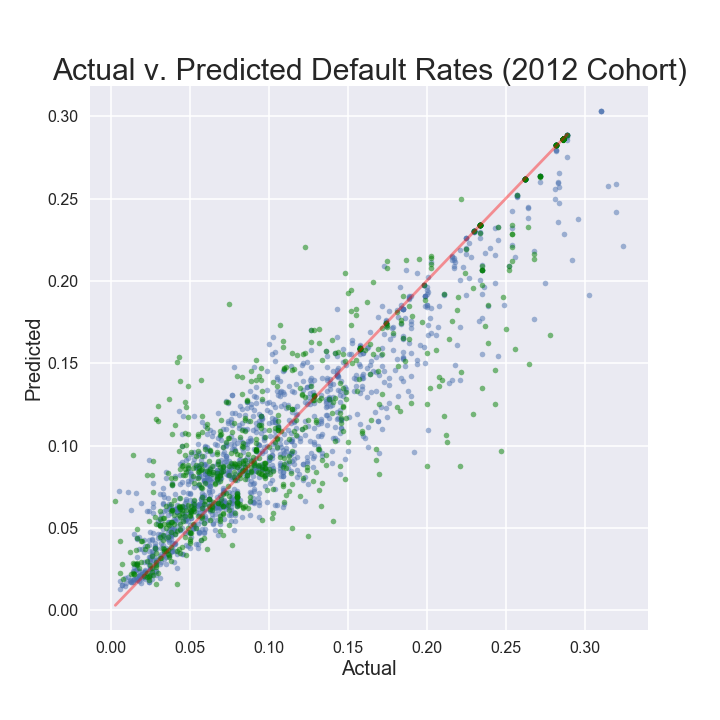
\includegraphics[width=2.5in]{results2012.png}
  \end{center}

  \caption{\Figure 3: Results of the model trained on data from the 2012 cohort}
  \label{results2012}
\end{figure}

\begin{figure}[!t]
  \begin{center}
    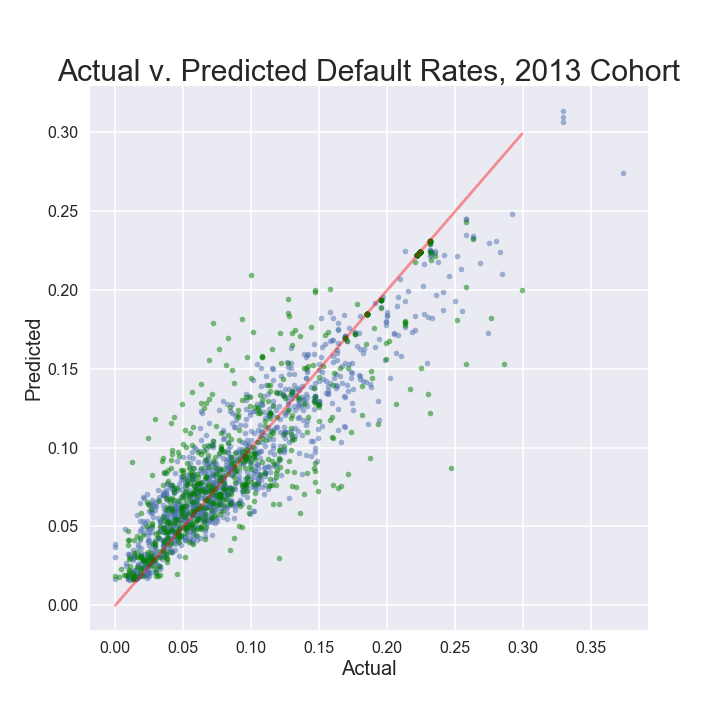
\includegraphics[width=2.5in]{results2013.png}
  \end{center}

  \caption{\Figure 4: Results of the model trained on data from the 2013 cohort}
  \label{results2013}
\end{figure}

\begin{figure}[!t]
  \begin{center}
    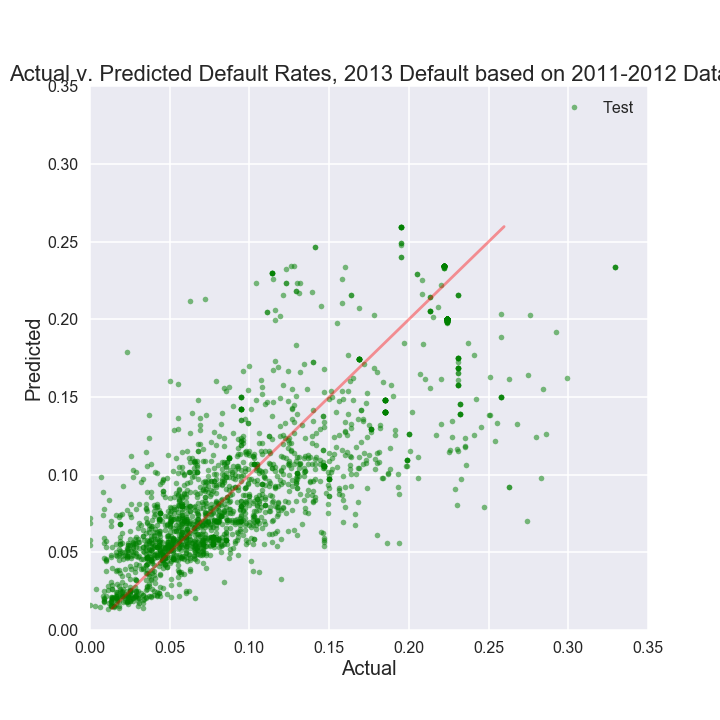
\includegraphics[width=2.5in]{2013from2011.png}
  \end{center}

  \caption{\Figure 5: Results of the model trained on data from the 2011 cohort
  and tested on the 2013 cohort}
  \label{results2013}
\end{figure}

\begin{figure}[!t]
  \begin{center}
    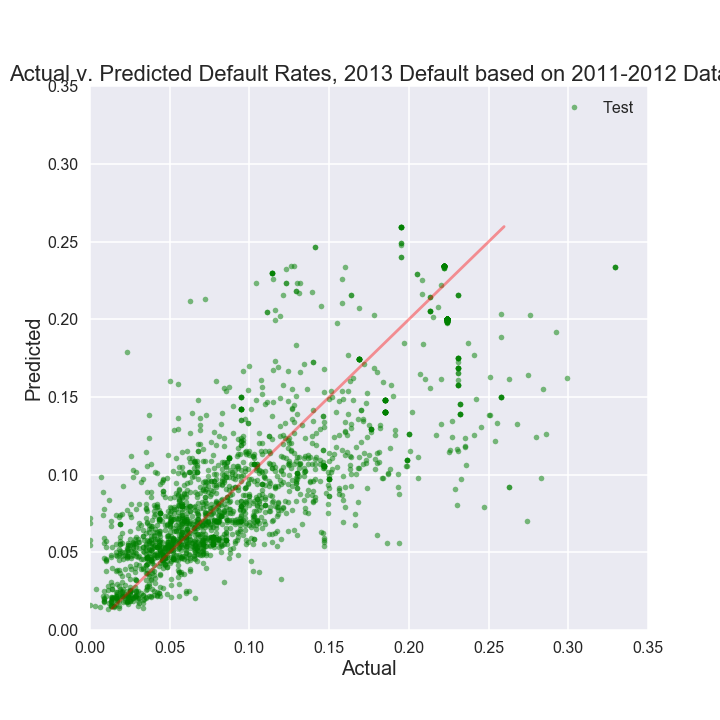
\includegraphics[width=2.5in]{2013from2011.png}
  \end{center}

  \caption{\Figure 6: Results of the model trained on averaged data from 2011-2012 cohorts
  and tested on the 2013 cohort}
  \label{resultsavg}
\end{figure}

\noindent\textbf{PS 1.} The file \texttt{refs.bib} contains the bibliographic references (see example).\\

\noindent\textbf{PS 2.} To generate a pdf you should run
\begin{enumerate}
\item pdflatex <file-name.tex>
\item bibtex <file-name> (without .tex)
\item pdflatex <file-name.tex>
\item pdflatex <file-name.tex>
\end{enumerate}


\bibliographystyle{abbrv}
\bibliography{refs}
\end{document}
